% Source: Code/xband-radar-sim/docs/radar_simulation_technical.tex
% Description: Ray-triangle intersection. The ray from origin $\mathbf{O

\documentclass[border=4pt]{standalone}
\usepackage{algpseudocode}
\usepackage{amsmath,amssymb,amsfonts}
\usepackage[T1]{fontenc}
\usepackage{graphicx}
\usepackage{pgfplots}
\usepackage{tikz}
\usepackage{xcolor}
\pgfplotsset{compat=1.18}
\usetikzlibrary{arrows.meta,positioning,shapes.geometric,calc,patterns,decorations.pathmorphing,3d,angles,quotes}

\definecolor{radargreen}{RGB}{0,255,0}
\definecolor{raycolor}{RGB}{255,165,0}
\definecolor{targetcolor}{RGB}{255,0,0}
\definecolor{groundcolor}{RGB}{139,90,43}
\definecolor{skycolor}{RGB}{135,206,235}
\definecolor{beamcolor}{RGB}{255,255,0}


\pgfmathsetmacro{\randx}{0.3*rand}
\pgfmathsetmacro{\y}{-1.1 + 2.2*rand}
\pgfmathsetmacro{\randx}{0.2*rand}

\begin{document}
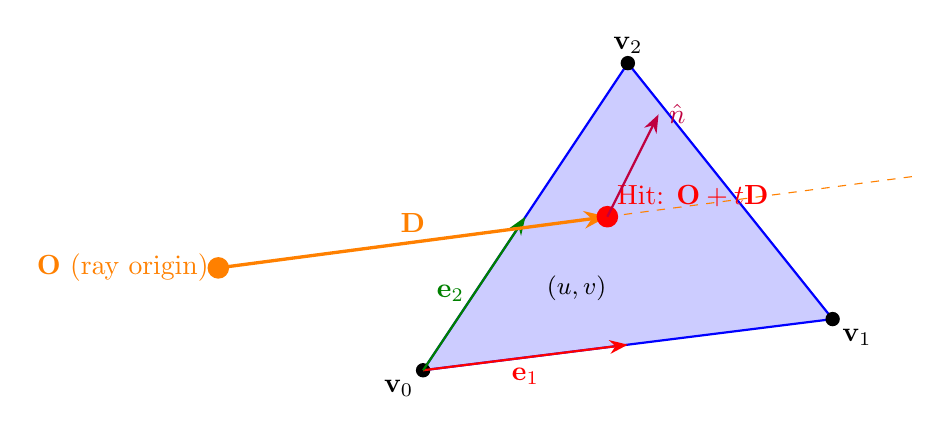
\begin{tikzpicture}[scale=1.3]
    % Triangle
    \coordinate (v0) at (0,0);
    \coordinate (v1) at (4,0.5);
    \coordinate (v2) at (2,3);

    \fill[blue!20] (v0) -- (v1) -- (v2) -- cycle;
    \draw[thick, blue] (v0) -- (v1) -- (v2) -- cycle;

    % Vertex labels
    \fill (v0) circle (2pt) node[below left] {$\mathbf{v}_0$};
    \fill (v1) circle (2pt) node[below right] {$\mathbf{v}_1$};
    \fill (v2) circle (2pt) node[above] {$\mathbf{v}_2$};

    % Edge vectors
    \draw[-{Stealth}, thick, red] (v0) -- ($(v0)!0.5!(v1)$) node[midway, below] {$\mathbf{e}_1$};
    \draw[-{Stealth}, thick, green!50!black] (v0) -- ($(v0)!0.5!(v2)$) node[midway, left] {$\mathbf{e}_2$};

    % Ray
    \coordinate (O) at (-2,1);
    \coordinate (hit) at (1.8,1.5);

    \fill[orange] (O) circle (3pt) node[left] {$\mathbf{O}$ (ray origin)};
    \draw[-{Stealth}, very thick, orange] (O) -- (hit);
    \draw[orange, dashed] (hit) -- ($(O)!1.8!(hit)$);
    \node[orange, above] at ($(O)!0.5!(hit)$) {$\mathbf{D}$};

    % Hit point
    \fill[red] (hit) circle (3pt) node[above right] {Hit: $\mathbf{O} + t\mathbf{D}$};

    % Normal vector
    \draw[-{Stealth}, thick, purple] (hit) -- ($(hit)+(0.5,1)$) node[right] {$\hat{n}$};

    % Barycentric coords
    \node at (1.5,0.8) {\small $(u,v)$};

\end{tikzpicture}
\end{document}
